\documentclass[a4paper, 12pt]{report}

\renewcommand{\thesection}{\arabic{section}} 

\usepackage[utf8]{inputenc}
\usepackage[T1]{fontenc}
\usepackage[francais]{babel}
\usepackage{fullpage}
\usepackage{hyperref}
\usepackage{enumitem}
\usepackage{listings}
\usepackage{graphicx}
\lstset{language=Java,basicstyle=\footnotesize,breaklines=true}

\title{Rapport Projet Traitement d'Image Android}
\author{Cyril \bsc {CAULONQUE}}
\date {}

\begin{document}
\maketitle
\newpage
    \tableofcontents
\newpage
\section{Présentation}
Cette application permet d'appliquer des filtres basiques à des images prédéfinies ou provenant de la caméra. Elle permet aussi de les enregistrer dans la galerie. Elle demande 2 permisions : écrire dans la mémoire externe et prendre des photos. La version de l'api requise est la 23.\newline Le code de l'application comporte 4 activités : \emph{MainActivity, HistoActivity, KernelActivity, SelectColorActivity} et utilise 2 classes \emph{Traitement} et \emph{TouchImageView}, ainsi que 2 fichiers renderscript \emph{colorize.rs} et \emph{grey.rs}.\newline
L'activité main appelle toutes les autres. Toutes les fonctions de traitement d'image sont situées dans \emph{Traitement.java}.
A l'ouverture l'application propose 5 images, situées dans le dossier ressources. Dans le code, elles sont stockées dans un ArrayList de Bitmaps, car on veut pouvoir ajouter des bitmaps à celles déjà disponibles. L'image affichée à l'écran est la bitmap \emph{mutableBitmap}, l'image de base est stockée dans \emph{image\_bitmap} afin de pouvoir annuler les modifications à tout moment.
\section{Les algorithmes}
\subsection{Les algorithmes basiques}
Les algorithmes basiques proposés par l'application sont :\newline
\begin{itemize}
\item griser
\item griser + extension de l'histogramme
\item coloriser (teinte au hasard dans le format hsv)
\item noir \& blanc (bicolore)
\item filtrer (griser toutes les couleurs trop éloignées de la couleur sélectionné (Distance Euclidienne))
\begin{lstlisting}[frame=single]
distance = (int) Math.sqrt(Math.pow((R0 - R), 2) + Math.pow((G0 - G), 2) + Math.pow((B0 - B), 2));
if (distance > seuil) {
    greylvl = (R + G + B) / 3;
    pixels[k] = (255 & 0xff) << 24 | (greylvl & 0xff) << 16 | (greylvl & 0xff) << 8 | (greylvl & 0xff);
}
\end{lstlisting}
\item extension de l'histogramme sur les 3 canaux RGB.
\item égalisation. On crée une lookuptable avec les niveaux de gris et on l'applique ensuite aux 3 couleurs.
\end {itemize}
\subsection{Les convolutions}
Les algorithmes de convolutions sont :
\begin{itemize}
\item flou (taille variable) Les coefficients sont tous les mêmes.
\item flou gaussien (taille variable) Les coefficients sont répartis de manière plus circulaire :
\begin{lstlisting}
coeff = Math.exp(-((double) (x * x + y * y) / ((double) (2 * n * n))));
\end{lstlisting}
n étant la rayon du noyau. x et y la posiition du coefficient au sein du noyau.
\item gradient. La racine de $gradientX^2 + gradientY^2$. Valeur ramenée entre 0 et 255.
\item laplace. Assez semblable au gradient mais noyau différent :
\begin{lstlisting}
noyaulaplace = {{0, 1, 0}, {1, -8, 1}, {0, 1, 0}};
\end{lstlisting}
\end {itemize}
Les bords sont traités en reflétant l'image.
\subsection{Renderscript}
Il y a 2 scripts renderscript : 1 pour la fonction griser qui apporte une différence négligeable ( 133 639 micro secs réduit à 100 607 micro secs). La fonction la plus lente était la fonction colorize (chaque pixel est passé du format rgb au format hsv puis à nouveau rgb) avec un temps d'exécution de 10 340 087 micro secs. La version renderscript dure 339 104 micro secs, elle est donc 30 fois plus rapide.
\section{Fonctionnalités Supplémentaires}
\subsection{Visualiser l'histogramme}
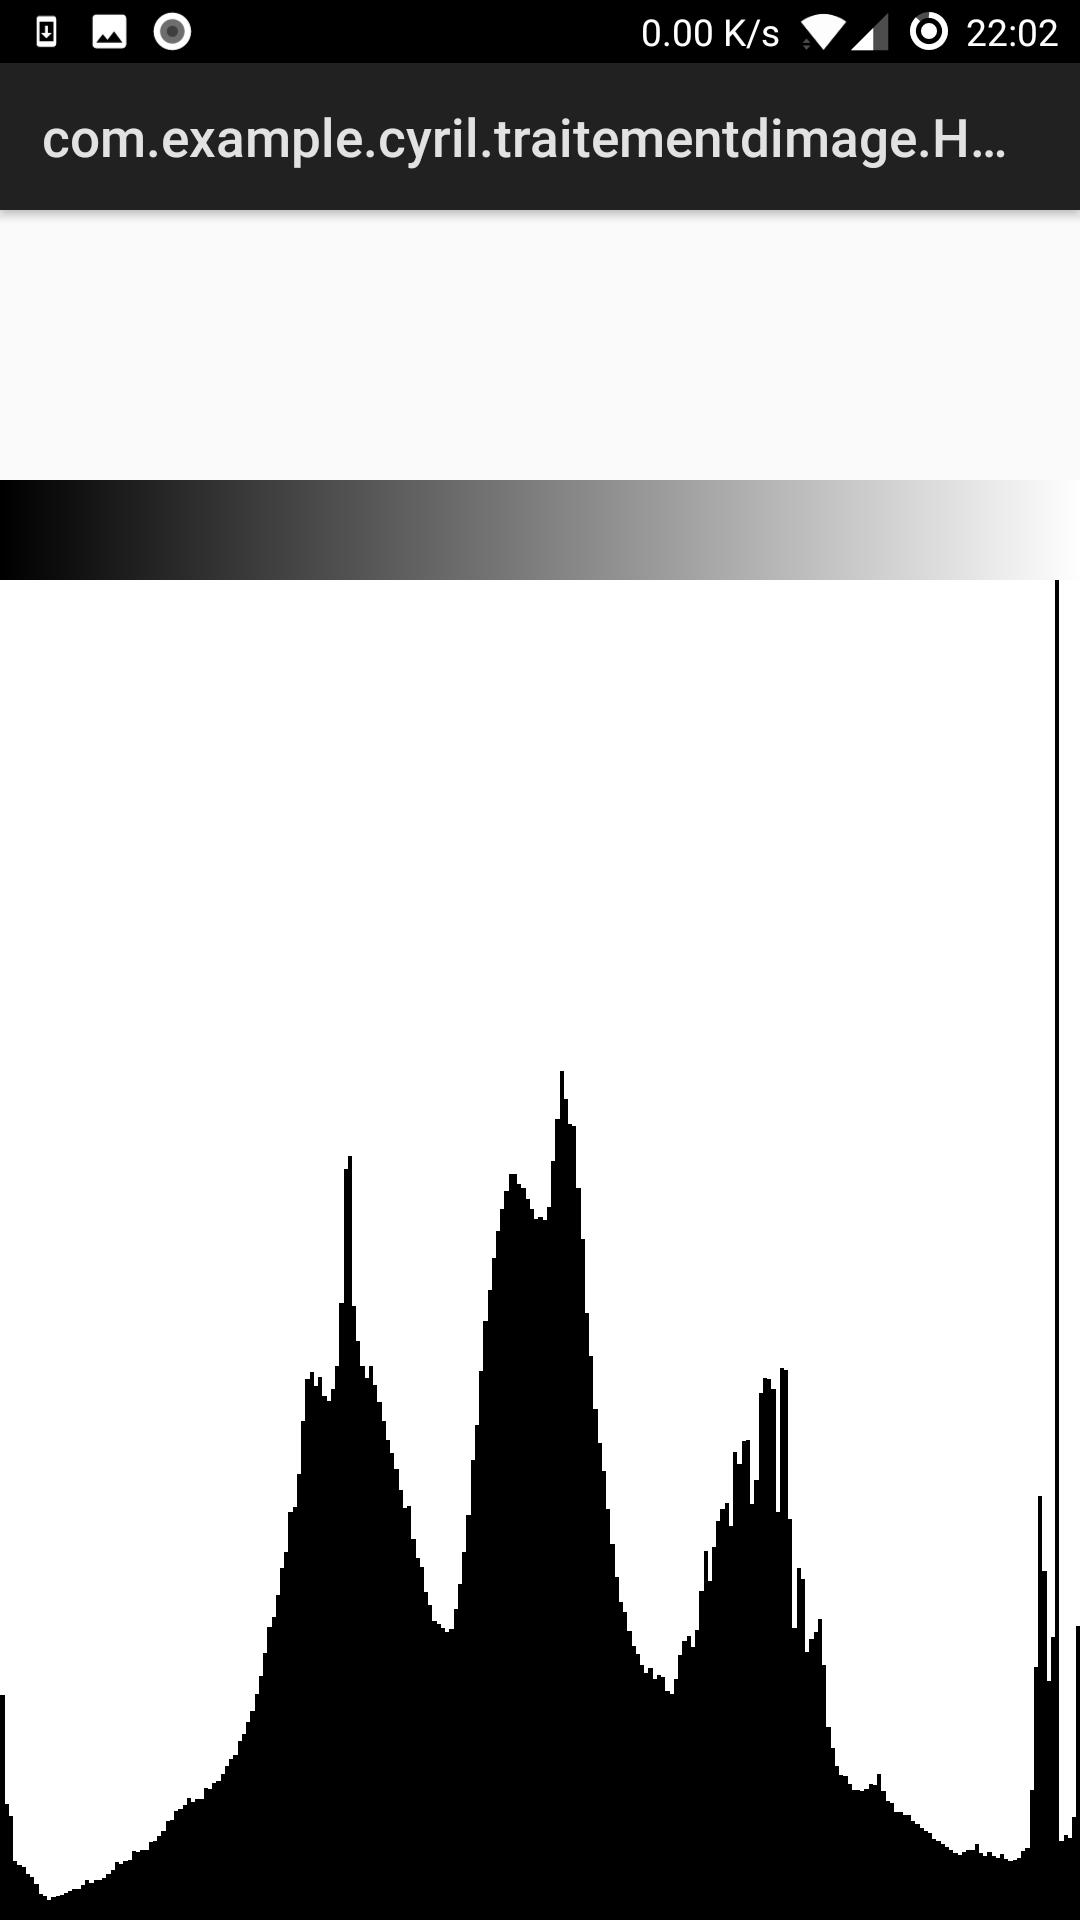
\includegraphics[width=5cm,scale=1]{ressources/histo.jpg}
\subsection{Prendre une photo}
L'application permet de prendre une photo, celle ci est ajoutée à la fin de l'ArrayList des bitmaps, peut donc être modifiée comme une image classique.
\subsection{Sélectionner une couleur (ou une taille)}
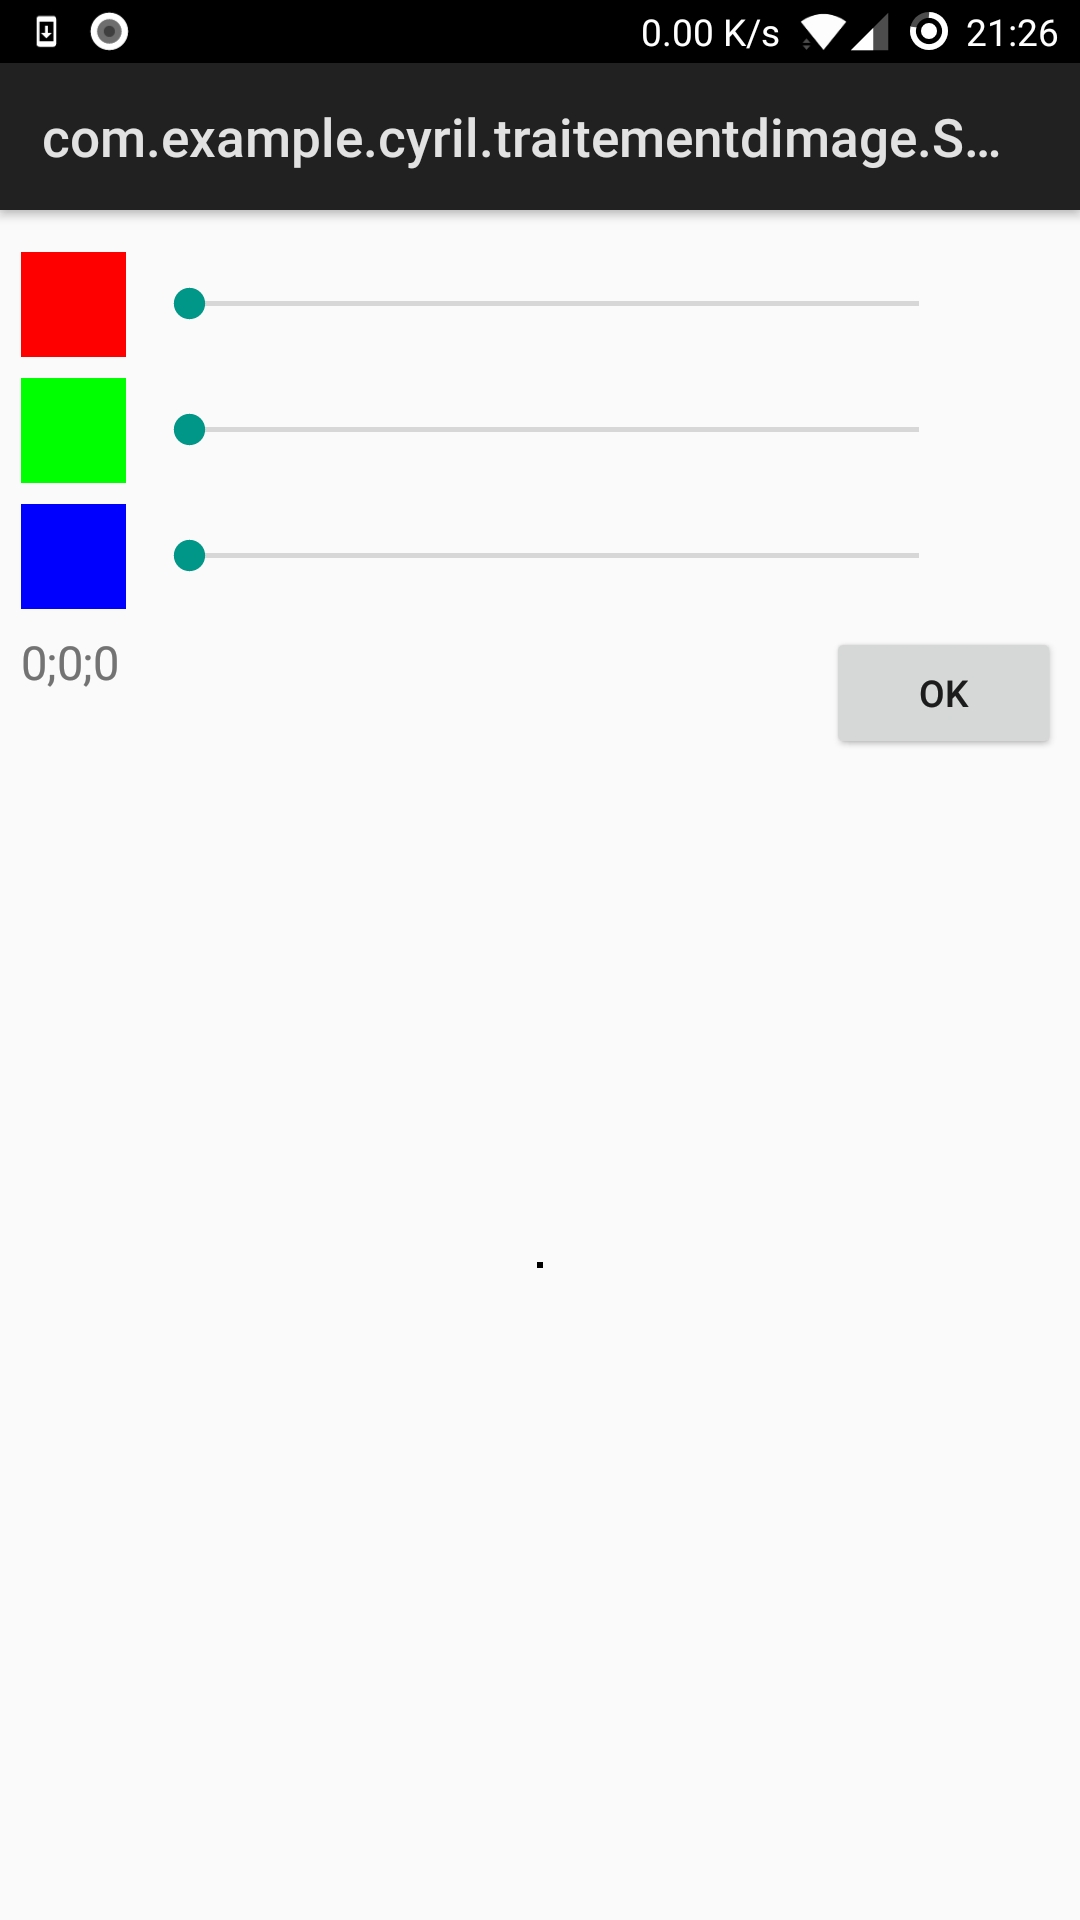
\includegraphics[width=5cm,scale=1]{ressources/select1.jpg}
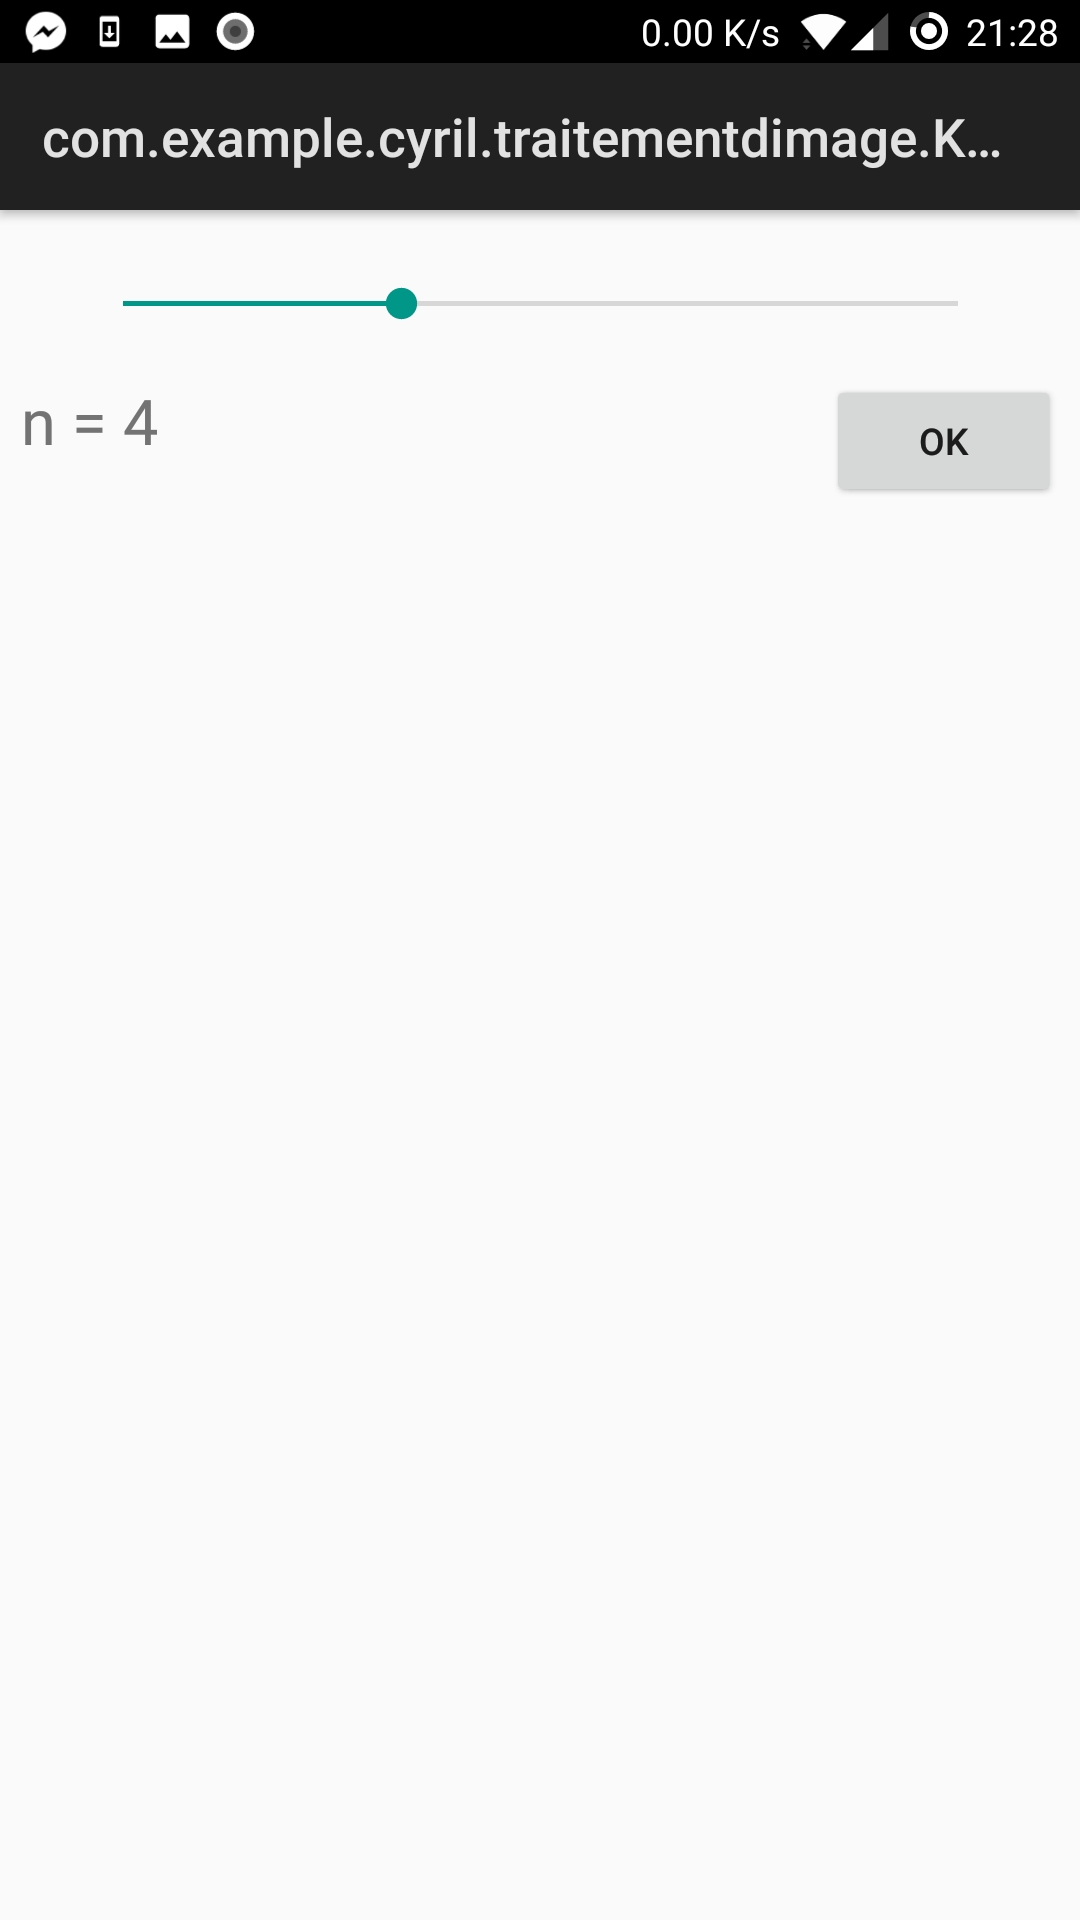
\includegraphics[width=5cm,scale=1]{ressources/select2.jpg}
\newline Il est possible de sélectionner une couleur pour la fonction "filtrer" (qui était à la base choisie aléatoirement), et de choisir la taille du kernel pour les fonctions de flou.
\subsection{Zoom au doigt}
La fonctionnalité de zoom au doigt utilise à 100\% une classe importée depuis un projet github. J'avais mes propres fonctions mais elles n'étaient pas totalement fonctionnelles, je n'arrivais pas à centrer le zoom sur le point entre les 2 doigts malgré de nombreuses tentatives et solutions différentes. J'ai donc décidé d'utiliser la classe TouchImageView.java trouvée sur internet.
\subsection{Sauvegarder une image}
L'application demandera la permission à l'utilisateur d'écrire dans la mémoire. Si la réponse est positive alors l'image en cours est enregistrée dans un sous dossier du dossier Pictures. Le fichier est nommé selon la date et l'heure.
\end{document}
